\Chapter{Felhasználói kézikönyv}

A fejezet a játék felhasználóknak készített kézikönyvét mutatja be.

\Section{A játék rövid leírása}

A játék egy ingatlankereskedelmi játék, melyben a játékosok az alaptőkéjüket ingatlanok adásával, vételével és bérbeadásával tudják növelni. Az győz, aki a játék végén a legtöbb vagyont gyűjtötte össze. Ehhez jó taktikára, üzleti érzékre illetve meggyőzőkészség szükséges. A START felíratú mezőről indulva mindenden játékos egyenlő tőkével kezdheti a játékot. A haladás ütemét kockadobás határozza meg. Különböző típusú mezőkre lépve más-más lehetőségeket kínálnak a játékosoknak. Vannak mezők, melyeken ingatlanokat lehet vásárolni, majd bérbeadni, a szerencsekártyák pedig előnyhöz vagy hátrányhoz is juttathatnak. De vigyázz! Így akár börtönbe is kerülhetsz. 

\Section{A játék kezdete}

Az alábbiakban felsorolásra kerül néhány fontosabb tudnivaló a játék indítás menetével kapcsolatosan.

\begin{itemize}
\item Az alkalmazás indítása után nevet és karaktert választ a játékos.
\item Az elsőnek belépő játékos lesz a host (a szoba irányítója), aki dönt a játék indításáról. Ha nincs meg a négy emberi játékos akkor a host tudja őket helyettesíteni különböző nehézségű szintű botokkal.
\item Az indítást követően kezdődhet a játék.
\item Minden játékos a "START" mezőről indul, 150.000 JF (JutiFalat) kezdőtőkével.
\end{itemize}

\Section{A játék menete}

A fordulód során dobj a kockáddal, aminek hatására új mezőre lépsz. A mező amelyikre érkezel meghatározza hogy mit kell tenned. Egy mezőn több játékos is állhat egyszerre.
\Aref{fig:fields}. ábrán látható mezők fordulnak elő.

\begin{figure}[h!]
\centering
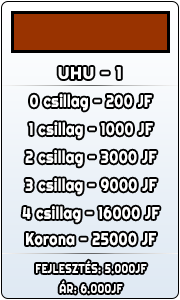
\includegraphics[scale=0.4]{images/p1.png}
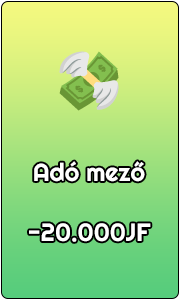
\includegraphics[scale=0.4]{images/ado.png}

\includegraphics[scale=0.4]{images/szk.png}
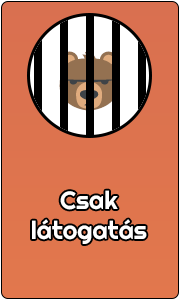
\includegraphics[scale=0.4]{images/bori_latogatas.png}

\includegraphics[scale=0.4]{images/parkolo.png}
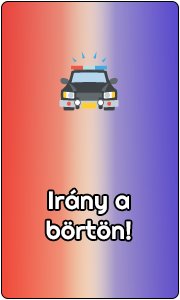
\includegraphics[scale=0.4]{images/bori.png}
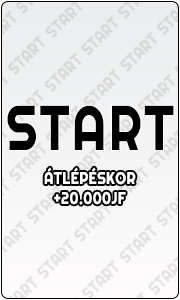
\includegraphics[scale=0.4]{images/start.png}
\caption{Játékban található mező kártyák}
\label{fig:fields}
\end{figure}

\begin{itemize}
	\item"Ingatlan" mező: Ha még nincs senkinek a birtokában, akkor megveheted azt. Ha már valakinek a tulajdonában van, akkor bérleti díjat kell fizetned.
	\item "Jövedelemadó" mező: A banknak adót kell fizetned, aminek az összege 20.000 JF.
	\item “Szerencsekártya" mező: Egy szerencsekártyát kapsz (ami nem biztos, hogy szerencse).
	\item "Börtön" mező: Ide csak látogatóba érkezel.
	\item "Ingyen parkoló" mező: Ez egy szimpla pihenő, semmilyen büntetéssel nem kell számolnod.
	\item "Irány a börtön!" mező: A "Börtön" mezőre kell lépned, ahol három körből kimaradsz. A "START" mező átlépéséért nem veheted át a jutalmad.
	\item"START" mező: Áthaladáskor, vagy rálépéskor 20.000 JF-ot kapsz.
\end{itemize}

\Section{Dupla dobás}

Abban az esetben, hogyha a játékos mindkét kockáján azonos szám szerepel, a szokott módon halad előre. Ezután újra dob a kockákkal, és továbblépve teljesíti az adott mező utasításait. Harmadszori dupla dobás esetén a játékos nem léphet egyet sem, illetve azonnal vége lesz a körnek, a következő játékos következik.

\Section{Ingatlanvásárlás}

Amennyiben a játékos olyan telekre lép, amely még senkinek nincs a birtokában jogában áll megvásárolni azt. Ha élni szeretne a vásárlás lehetőségével, abban az esetben a számlájáról levonásra kerül az ingatlan vételára cserébe megkapja az ingatlanhoz járó tulajdoni kártyát. Azonban a játékos dönthet úgy is, hogy nem vásárolja meg az ingatlant, ebben az esetben nem kell bérleti díjat fizetnie senkinek, továbbá befejezheti a körét.

\Section{Megvásárolt ingatlanok}

Hogyha a játékos rendelkezik tulajdoni kártyával valamely ingatlanhoz, majd egy másik játékos arra ingatlan mezőre rálép köteles bérleti díjat fizetni az ingatlan tulajdonosának.

A telek fejlesztése kizárólag abban az esetben lehetséges, hogyha az összes azonos színű teleknek a tulajdonosa a játékos. Két fajta fejlesztéssel lehet bővíteni az ingatlanokat: "Csillag" illetve "Korona". A "Korona" fejlesztés akkor válik elérhetővé, hogyha az adott ingatlan rendelkezik 4 db "Csillag" fejlesztéssel. Ezeknek a megvételéhez szükséges összeg megtalálható az ingatlanhoz tartozó kártyákon.

Törekedj arra, hogy minél előbb juss hozzá ezekhez, hiszen csak 32 db "Csillag" illetve 12 db "Korona" fejlesztés érhető el a játék folyamán. Abban az esetben, ha valamelyik játékos továbbfejleszt egy 4 "Csillag" fejlesztéssel rendelkező ingatlant egy "Korona" fejlesztéssé, a "Csillag"-ok visszakerülnek a megvásárolhatók közé. Érdemes nagy hangsúlyt fektetni az ingatlanok fejlesztésére, hiszen ez növeli a bérleti díj költségét.

Fejleszteni mindenkinek kizárólag a saját körében lehetséges.
Lehetőség van a már meglévő fejlesztéseket eladni, a tulajdoni kártyán szereplő összeg feléért a bank számára.

Két játékosnak lehetősége van egymás között eladni/cserélni ingatlanokat megegyezés szerint, viszont abban az esetben, hogyha az adott színcsoportba tartozó bármelyik ingatlanon fejlesztés található, kötelező lebontani a csere előtt.

\Section{Közművek}

\begin{figure}[h!]
\centering
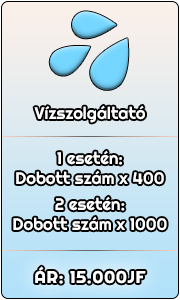
\includegraphics[scale=0.4]{images/vsz.png}
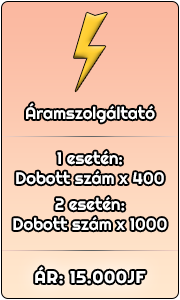
\includegraphics[scale=0.4]{images/asz.png}
\caption{Közmű kártyák}
\label{fig:ff}
\end{figure}

Az ilyen típusú mezőkre lépve a játékosnak lehetősége van megvásárolni a mezőn feltüntetett összegért, feltéve ha ezt még senki nem birtokolja. Ebben az esetben az összeg levonásra kerül a számlájáról. Ha már valaki másé, a játékos újra dob a kockákkal. Ha a közmű tulajdonosának csak egy közműve van, akkor a dobott szám négyszázszorosát, ha viszont mindkét közmű a birtokában áll, a dobott szám ezerszeresét kell kifizetni.

\Section{Cégek}

\begin{figure}[h!]
\centering
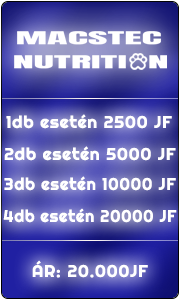
\includegraphics[scale=0.4]{images/b1.png}
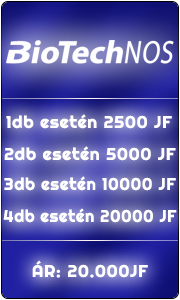
\includegraphics[scale=0.4]{images/b2.png}
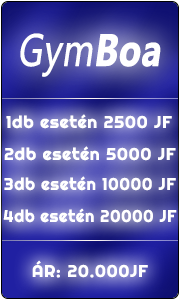
\includegraphics[scale=0.4]{images/b3.png}
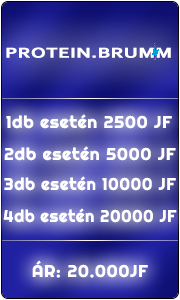
\includegraphics[scale=0.4]{images/b4.png}
\caption{Biznisz kártyák}
\label{fig:ff}
\end{figure}

Ha a játékos elsőként lép ilyen mezőre, módjában áll megvásárolni az adott céget. Abban az esetben ha már más tulajdonában van az adott cég, a játékos köteles az ingatlankártyán feltüntetett összeget kifizetni a cég tulajdonosának.

\begin{itemize}
\item 1 cég birtoklása esetén: 2500 JF
\item 2 cég birtoklása esetén: 5000 JF
\item 3 cég birtoklása esetén: 10000 JF
\item 4 cég birtoklása esetén: 20000 JF
\end{itemize}

\Section{Börtön}

Ha a játékos börtönbe kerül, három fordulón keresztül kimarad a játékból. Minden körben megpróbálhat dobni, és abban az esetben hogyha duplát dob kijöhet ingyen a börtönből, majd dobott számút lép.

Az alábbi esetekben kerülsz börtönbe:

\begin{itemize}
\item "Irány a börtön!" mezőre lépsz
\item Ha olyan szerencsekártyát húztál, amin ez az utasítás áll.
\item Háromszor dobtál egymás után duplát.
\end{itemize}

A fordulód ezután rögtön véget ér. Ha a börtönbe vezető úton léptél át a "START" mezőn, nem kapod meg az érte járó fizettséget.

Hogyan juthatsz ki a börtönből:

\begin{itemize}
\item Fizess 5.000 JF-ot a következő körben és folytathatod a játékot.
\item Használd az "Ingyen szabadulhatsz a börtönből!" kártyát.
\item Próbálj meg duplát dobni.
\end{itemize}

\Section{Csőd, a játék vége}

Abban az esetben ha a játékos nem tudja kifizetni a bankot, vagy bármely másik játékost, csődöt kell jelenteni. Ekkor a játékos kiesett a játékból. A játék addig tart amíg az első két játékos csődöt nem jelent. Ezután a szerver összesíti a maradék játékosok vagyonait és az lesz a győztes, aki a legnagyobb összeggel rendelkezik.

